\section{Quintic: degree=5}
\label{sec.quintic}

This exercise is left as an exercise for the student.  However, the following are some
notes to help lead the student in the right direction.

\begin{figure}
\centering
%% derived from https://tex.stackexchange.com/questions/357538/graph-of-a-parabola-on-pgfplots
%% Thanks to Stefan Pinnow
%%     https://tex.stackexchange.com/users/95441/stefan-pinnow

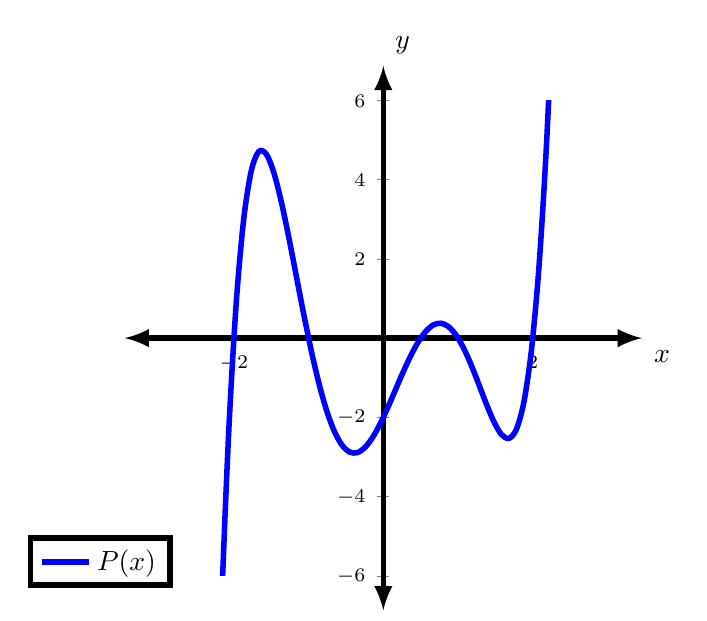
\begin{tikzpicture}
  \begin{axis}[
      samples=70,
      smooth,
      line width=2pt,
      domain=-4:3,
      legend pos=south west,
      legend style={
        anchor=east
      },
      width=0.6\textwidth,
      height=3in,
      axis lines=middle,
      xmin=-3,
      xmax=3,
      ymin=-6,
      ymax=6,
        scaled ticks=false,
        ticklabel style={font=\scriptsize},
        xlabel=$x$,
        ylabel=$y$,
        axis line style={
          latex-latex,
          shorten >=-12.5pt,
          shorten <=-12.5pt,
        },
        xlabel style={at={(ticklabel* cs:1)}, xshift=12.5pt, anchor=north west},
        ylabel style={at={(ticklabel* cs:1)}, yshift=12.5pt, anchor=south west},
    ]
    
    \addplot[color=blue] {x^5 - 0.5 * x^4 - 5* x^3 + 2.5 * x^2 + 4* x - 2};  
    \addlegendentry{\(P(x)\)}
  \end{axis}
\end{tikzpicture}
%

\caption{Quintic}
\label{fig.quintic}
\end{figure}

\begin{align*}
  P(x) &= x^5 - \frac{1}{2} x^4 + 5 x^3 + \frac{5}{2} x^2 + 4 x - 2
\end{align*}


A quintic polynomial has the form $P(x) = a x^5 + b x^4 + c x^3 + d x^2 + e x + f$.
If $a=0$ then $P(x)$ is really
a quartic polynomial (degree~4) and can be solved using the techniques described in Section~\ref{sec.quartic}.
Since a quintic polynomial has odd degree (if $a\neq 0$),
then, like the cubic (Section~\ref{sec.cubic}), it is guaranteed to have a real root.  This fact
is guaranteed, because if
$a>0$ then $P(x)\to \infty$ for $x>>0$ and $P(x)\to -\infty$ for $x<<0$.

Given this fact, we can find a root, $r$ using a binary search as we did for the cubic.
Since $P(0) = f$, then we can consider two cases.
\begin{enumerate}
\item If $f>0$ then search for a root on the negative x-axis
\item If $f<0$ then search for a root on the positive x-axis
\end{enumerate}

Once the root $r$ is found, factor out $(x-r)$ from $P(x)$ to result in a quartic, which we can solve using
the technique in Section~\ref{sec.quartic}.
\begin{align*}
  P(x) &= a x^5 + b x^4 + c x^3 + d x^2 + e x + f\\
  &= (x - r) (Ax^4 + B x^3 + C x^2 + D x + E)
\end{align*}

Where

\begin{align*}
  A &= a\\
  B &= b + a r\\
   &= b + A r\\
  C &= c + b r + a r^2\\
  &= c + (b + a r)r\\
  &= c + B r\\
  D &= d + c r + b r^2 + a r^3\\
  &= d + ( c + b r + a r^2)r\\
  &= d + C r\\
  E &= e + d r + c r^2 + b r^3 + a r^4\\
  &= e + ( d + c r + b r^2 + a r^3)r\\
  &= e + D r
\end{align*}


Having determined $A$, $B$, $C$, $D$, and $E$, the roots of
\[A x^4 + B x^3 + C x^2 + D x + E\] can be
found with a call to \code{find\_quartic\_roots}, which you implemented in Section~\ref{sec.quartic}.



% LocalWords:  Quintic quintic quartic
